
\documentclass[class={IEEEtran}]{standalone}

\usepackage{amsmath}
\usepackage{tikz}
\usepackage{pifont}

\newcommand{\whiteding}[1]{\large{\ding{\numexpr171+#1\relax}}}
\pagestyle{empty}
\usetikzlibrary{shapes.geometric,shapes.arrows,positioning,calc,arrows.meta,math}

\tikzset{AGENT/.style={rectangle,minimum width=6.5em,minimum height=3.5ex,draw,semithick,align=flush center}}
\tikzset{NOTE/.style={rectangle,rounded corners,draw,semithick,align=flush center,fill=white}}
\tikzset{ARROW/.style={thick, -stealth}}
\tikzset{DARROW/.style={<->,>={Triangle Cap[cap angle=90]}, line width=4ex, gray!20 }}

\begin{document}
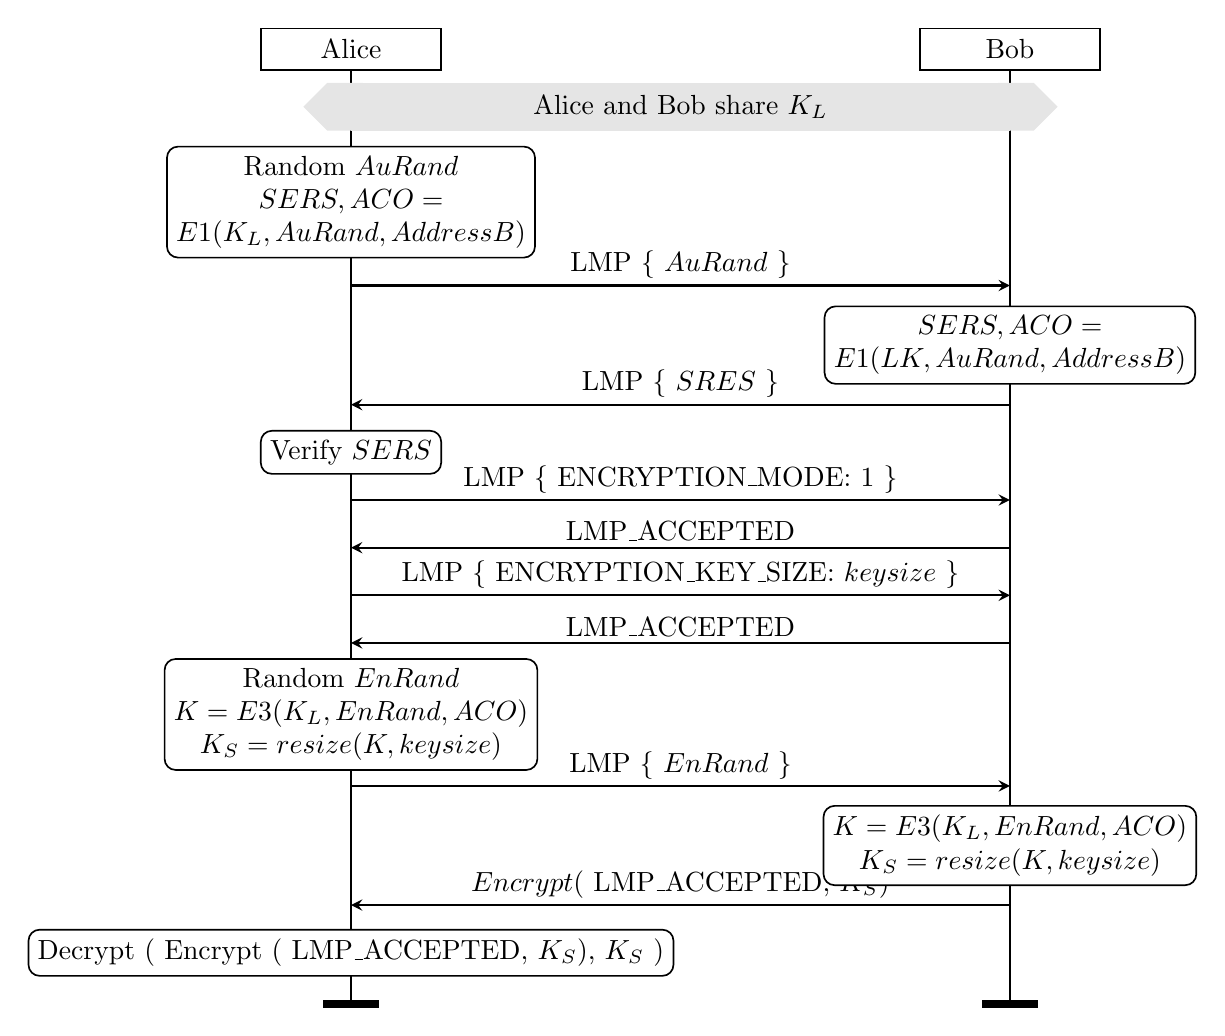
\begin{tikzpicture}

\node[AGENT] (n_alice) {Alice};
\node[AGENT, right=0.5\textwidth of n_alice] (n_bob) {Bob};

\coordinate (c_0_0) at ($(n_alice.south)+(0,-18ex)$);
\coordinate (c_0_1) at ($(c_0_0-|n_bob)$);
\draw[ARROW] (c_0_0) -- (c_0_1) node[midway,above=-0.3ex]{LMP \{ $AuRand$ \}};

\coordinate (c_1_0) at ($(c_0_1)+(0,-10ex)$);
\coordinate (c_1_1) at ($(c_1_0-|n_alice)$);
\draw[ARROW] (c_1_0) -- (c_1_1) node[midway,above=-0.3ex]{LMP \{ $SRES$ \}};

\coordinate (c_2_0) at ($(c_1_1)+(0,-8ex)$);
\coordinate (c_2_1) at ($(c_2_0-|n_bob)$);
\draw[ARROW] (c_2_0) -- (c_2_1) node[midway,above=-0.3ex]{LMP \{ ENCRYPTION\_MODE: 1 \}};

\coordinate (c_3_0) at ($(c_2_1)+(0,-4ex)$);
\coordinate (c_3_1) at ($(c_3_0-|n_alice)$);
\draw[ARROW] (c_3_0) -- (c_3_1) node[midway,above=-0.3ex]{LMP\_ACCEPTED};

\coordinate (c_4_0) at ($(c_3_1)+(0,-4ex)$);
\coordinate (c_4_1) at ($(c_4_0-|n_bob)$);
\draw[ARROW] (c_4_0) -- (c_4_1) node[midway,above=-0.3ex]{LMP \{ ENCRYPTION\_KEY\_SIZE: $keysize$ \}};

\coordinate (c_5_0) at ($(c_4_1)+(0,-4ex)$);
\coordinate (c_5_1) at ($(c_5_0-|n_alice)$);
\draw[ARROW] (c_5_0) -- (c_5_1) node[midway,above=-0.3ex]{LMP\_ACCEPTED};

\coordinate (c_6_0) at ($(c_5_1)+(0,-12ex)$);
\coordinate (c_6_1) at ($(c_6_0-|n_bob)$);
\draw[ARROW] (c_6_0) -- (c_6_1) node[midway,above=-0.3ex]{LMP \{ $EnRand$ \}};

\coordinate (c_7_0) at ($(c_6_1)+(0,-10ex)$);
\coordinate (c_7_1) at ($(c_7_0-|n_alice)$);
\draw[ARROW] (c_7_0) -- (c_7_1) node[midway,above=-0.3ex]{$Encrypt$( LMP\_ACCEPTED, $K_S$)};

\coordinate (c_end_0) at ($(c_7_1-|n_alice)+(0,-8ex)$);
\draw[semithick] (n_alice.south) -- (c_end_0);
\draw[fill=black] ($(c_end_0)+(-1em,0)$) rectangle ($(c_end_0)+(1em,-0.6ex)$);

\coordinate (c_end_1) at ($(c_end_0-|n_bob)$);
\draw[semithick] (n_bob.south) -- (c_end_1);
\draw[fill=black] ($(c_end_1)+(-1em,0)$) rectangle ($(c_end_1)+(1em,-0.6ex)$);


\draw[DARROW] ($(n_alice.south)+(-4ex,-3ex)$) to node[black,sloped]{Alice and Bob share $K_L$} ($(n_bob.south)+(4ex,-3ex)$);

\node[NOTE,minimum height=3.5ex] (n_alice1) at ($(n_alice.south)+(0,-11ex)$) {Random $AuRand$ \\ $SERS, ACO = $\\$E1(K_L, AuRand, AddressB)$};

\node[NOTE,minimum height=3.5ex] (n_bob1) at ($(c_0_1)+(0,-5ex)$) {$SERS, ACO = $\\$E1(LK, AuRand, AddressB)$};

\node[NOTE,minimum height=3.5ex] (n_alice2) at ($(c_1_1)+(0,-4ex)$) {Verify $SERS$};

\node[NOTE,minimum height=3.5ex] (n_alice3) at ($(c_5_1)+(0,-6ex)$) {Random $EnRand$ \\ $K = E3(K_L, EnRand, ACO)$ \\ $K_S = resize(K, keysize)$};

\node[NOTE,minimum height=3.5ex] (n_bob2) at ($(c_6_1)+(0,-5ex)$) {$K = E3(K_L, EnRand, ACO)$ \\ $K_S = resize(K, keysize)$};

\node[NOTE,minimum height=3.5ex] (n_alice4) at ($(c_7_1)+(0,-4ex)$) {Decrypt ( Encrypt ( LMP\_ACCEPTED, $K_S$), $K_S$ )};




% \node[NOTE,minimum height=3.5ex] (n_bob_1) at ($(c_0_1)+(0,-4ex)$) 
%     { $SERS = E1(LK, AuRand, AddressB)[0,...,3]$ \\ 
%       $ACO = E1(LK, AuRand, AddressB)[4,...,15]$ };

\end{tikzpicture}
\end{document}
